\documentclass[12pt]{article}
\usepackage[utf8]{inputenc}
\usepackage[paper=letterpaper,margin=1.25in]{geometry}
\usepackage{graphicx} 
\graphicspath{ {figures/} } % all figures are in the 'figures' folder
\usepackage{float}
\usepackage{indentfirst}
\usepackage{setspace}
\usepackage{amsmath}

% set up clickable links in ToC
\usepackage{hyperref}
\hypersetup{linktocpage, colorlinks=false, linktoc=all}
% add in dots for sections in ToC
\usepackage{tocloft}
\renewcommand\cftsecleader{\cftdotfill{\cftdotsep}}
% include subsections, etc.. in table of contents
\setcounter{tocdepth}{4}
\setcounter{secnumdepth}{4}

% verilog code snippet configuration
\usepackage[usenames,dvipsnames,svgnames,table]{xcolor}
\usepackage{listings}
\lstset{
	language=Verilog,
	frame=single,
	numbers=left,
	keywordstyle=\color{Blue}\ttfamily\footnotesize,
        commentstyle=\color{Green}\ttfamily\footnotesize,
	}  

\begin{document}

% turn off page numbering for the first few pages
\pagenumbering{gobble}

%%%% Title page %%%%
\begin{titlepage}
	\centering
	%{\huge\bfseries Real-Time Remote Mapping\par}
	{\huge\bfseries FPGA-Based Real-Time SLAM\par}
	\vfill
	
\includegraphics[width=7cm]{WPI_Inst_Prim_FulClr.png} % also works with logo.pdf
	\vfill
	{\par\large A Major Qualifying Project Report Submitted to the Faculty of \par}
	\vspace{0.25cm}
	{\large Worcester Polytechnic Institute\par}
	\vfill
	{\large In partial fulfillment of the requirements for the \par}
	\vspace{0.25cm}
	{\large Degree of Bachelor of Science in Electrical \& Computer Engineering\par}
	\vfill
	{\large By: \par}
	\vspace{0.25cm}
	{\Large Georges Gauthier \\ John DeCusati \par} 
	\vfill
	{\large \today \par}
	\vfill
	{\begin{flushright} 
	\large Advisor: \\ \Large Professor R. James Duckworth
	\end{flushright}}
\end{titlepage}
\newpage

% change margins, set to double space
\newgeometry{top=1in,bottom=1in,right=1in,left=1in}
\doublespacing

% create a table of contents
\tableofcontents
\newpage

%create a list of figures
\listoffigures
\newpage 

\pagenumbering{roman} % change page numbering to i,ii, ...

%%%% Acknowledgements %%%%
%\phantomsection % makes clickable ToC link work
\addcontentsline{toc}{section}{Acknowledgements}
\section*{Acknowledgements}
text
%\newpage

%%%% Abstract %%%%
\phantomsection
\addcontentsline{toc}{section}{Abstract}
\section*{Abstract}
The overall goal of this project is to create a device capable of generating detailed maps and imagery of an area in real-time. This device will rely on an FPGA, and will use image processing algorithms capable of detecting, localizing, and tracking human beings. The device will gather imagery from the visual light and infrared-spectrums, as well as localization data and distance measurements from an IMU and a rangefinder. Along with gathering and processing data, the device will also serve as a long-range wireless access point, and will be able to transmit all generated maps and imagery in real-time. A major deliverable of this project is that the transmitted data will be fully processed, allowing it to be viewed remotely on less-powerful, mobile devices.
\par
This device will be especially useful for first responders. It is intended to be mounted on a small remote control vehicle, allowing any connected user to wirelessly traverse dangerous and remote locations in search of people in need. Since this device transmits data in real-time, it will be able to provide first responders with an accurate representation of not only a 2-D floor plan of an area such as a building, but also where any people are located. An anticipated use of this device would be in the event of a building in danger of collapsing. Since it would be dangerous to physically enter the building, first responders could locate any people trapped inside and find the fastest route to them using the wirelessly transmitted floorplan. The first responders would also be aware of any dangers in their way by making use of the real-time augmented video stream. This video stream will consist of image data with overlaid with object indicators and location information on any human beings detected by the image processing algorithms.
 

\newpage

\pagenumbering{arabic} % change page numbering to 1,2, ...

%%%% Introduction %%%%
\section{Introduction}
In recent years, improvements in embedded processing technology have allowed for the creation of robotic situational awareness platforms for remotely observing dangerous or inaccessible areas. The market for such devices is a new and expanding field, and faces large demand from the military and first responders. This field is being piloted by throwable and remotely drivable platforms such as the Endeavor Robotics 110 FirstLook and the Bounce Imaging Explorer, shown in Figure \ref{robocop}. 

\par
\begin{figure}[H]
        \begin{subfigure}[h]{0.5\textwidth}
             \centerline{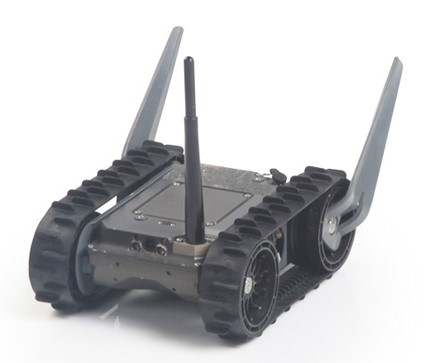
\includegraphics[width=1.0\textwidth]{FirstLook.jpg}}
            \caption{Endeavor Robotics 110 FirstLook \cite{endeavor}}
        \end{subfigure}
        \begin{subfigure}[h]{0.5\textwidth}
            \centerline{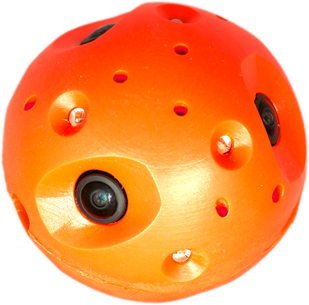
\includegraphics[width=0.8\textwidth]{bounce_img.png}}
            \caption{Bounce Imaging Explorer \cite{bounceImaging}}
        \end{subfigure}
\caption{Robotic Situational Awareness Devices}
\label{robocop}
\end{figure}
\par
These devices contain simple wireless video streaming technology, allowing for remote visual surveillance. Although a video stream is an effective strategy for simple surveillance, this method of gathering information has room for improvement. This project investigated the extraction of information such as object positioning and localization from a camera-based sensor suite in real time, allowing for more comprehensive situational observation. One method of performing this process is through the use of Simultaneous Localization and Mapping, or SLAM. 
\par
SLAM is a technique of mapping an unknown environment with respect to an agent, and can be performed using a wide variety of sensors and computational methods. This technique is a common area of research in the fields of image processing and high-speed computing, and has been applied mainly to autonomous vehicles. Most current SLAM implementations rely on the use of a sensor suite connected to a computer or System on Chip (SoC) computing device. 
\par
One type of technology useful for performing the high speed data processing necessary for an embedded SLAM device is a Field Programmable Gate Array, or FPGA. FPGAs consist of digital circuitry that is designed to be user-configured, allowing for the creation of completely customized digital hardware. FPGAs are especially useful for parallelized data processing, posing potential real-time advantages over standard computing or microcontroller technology. Although FPGA technology is highly applicable to performing SLAM-like tasks, there are currently few existing products that use FPGAs for this purpose. 
\par
This project explored the viability of an FPGA-based real-time SLAM sensor suite as a replacement for standard video cameras on existing situational awareness systems. This sensor suite utilized data from stereo camera modules, a scanning laser rangefinder, and an Inertial Measurement Unit (IMU) to create a real-time depth-augmented video feed and a 2D floorplan from the device's field of view.
\par
The following chapters detail the creation of this sensor suite, beginning with an exploration of relevant technology and prior work. Next, the overall system design of the project is included with a system block diagram. Then, each individual sensor’s implementation is explored in more detail. Methods for processing and combining sensor data to produce the intended 2D floorplan and 3D map visualizations are included. Comprehensive test results are then examined in detail for all sensors and main algorithms used. Lastly, conclusions and recommendations for future improvements are presented. 

\newpage

%%%% Bibliography %%%%

\singlespacing
%https://www.sharelatex.com/learn/Bibliography_management_with_bibtex
\begin{thebibliography}{9}

\bibitem{al422b}
Averlogic.
\textit{AL422B Data Sheets}. 2001.
Available from: \url{http://www.frc.ri.cmu.edu/projects/buzzard/mve/HWSpecs-1/Documentation/AL422B_Data_Sheets.pdf}.

\bibitem{davison} 
Davison, A.J.,
\textit{Real-Time Simultaneous Localisation and Mapping with a Single Camera}. 
IEEE Computer Vision, 2003. 2(1).

\bibitem{livm34lp}
Leopard Imaging Inc.
\textit{LI-VM34LP Camera Board}. 2009.
Available from: \url{http://www.leopardimaging.com/uploads/li-vm34lp_v1.1.pdf}.

\bibitem{serveball}
\textit{Serveball}.
Available from: \url{http://www.serveball.com/}.

\bibitem{mattoccia}
Stefano Mattoccia, M.P.,
\textit{A passive RGBD sensor for accurate and real-time depth sensing self-contained into an FPGA}.
in \textit{International Conference on Distributed Smart Cameras}. 2015.

\bibitem{mt9v032}
On Semiconductor. 
\textit{MT9V032: 1/3-Inch Wide-VGA CMOS Digital Image Sensor}. 2015. 
Available from: \url{http://www.onsemi.com/pub_link/Collateral/MT9V032-D.PDF}.

\bibitem{mt9v034}
On Semiconductor. 
\textit{MT9V034: 1/3-Inch Wide-VGA CMOS Digital Image Sensor}. 2015. 
Available from: \url{http://www.onsemi.com/pub_link/Collateral/MT9V034-D.PDF}.

\bibitem{porikli}
Fatih Porikli, O.T.,
\textit{Human Body Tracking by Adaptive Background Models and Mean-Shift Analysis}.
in \textit{IEEE International Workshop on Performance Evaluation of Tracking and Surveillance}. 2003.

\bibitem{thrun}
Sebastian Thrun, D.H., David Ferguson, Michael Montemerlo, Rudolph Triebel, and C.B. Wolfram Burgard, Zachary Omohundro, Scott Thayer, William Whittaker.
\textit{A System for Volumetric Robotic Mapping of Abandoned Mines}. 
in \textit{IEEE International Conference on Robotics and Automation}. 2003.

\end{thebibliography}

% include in ToC - must be after refs for correct page link from hyper
\addcontentsline{toc}{section}{References}
\doublespacing
\newpage

%%%% Example code - DELETE ME BEFORE FINAL SUBMISSION %%%%
\newpage
\subsection{LaTeX Coding Examples}
This section isn't intended to remain here, but can serve as an example for how to set things up later on

\subsubsection{Figures} 
\begin{figure}[H]
	\centerline{
\includegraphics[width=0.25\textwidth]{WPI_Inst_Prim_FulClr.png}}
	\caption{A Test Figure}
	\label{wpiLogo}
\end{figure}

Using the \verb!\ref! command, I'm able to reference Figure \ref{wpiLogo} by calling \verb!\ref{wpiLogo}!.

\subsubsection{Code Snippet}
Code snippets can be created by calling \verb!\begin{lstlisting}!, inserting all code, and then calling \verb!\end{lstlisting}!. Also call \verb!\singlespacing! before the code snippet and \verb!\doublespacing! after to keep things from getting too big.
\singlespacing % single space code
\begin{lstlisting}
//verilog code example
always @ (x, y, z)
  x <= y + z;
\end{lstlisting}
\doublespacing % return to double spacing after

\subsubsection{Using the bibliography}
All bibliographic references are contained in \texttt{bib.tex}. To cite a reference in the paper, use the \verb!\cite! command.
\par
As an example, I can cite \textit{Serveball} at the end of this sentence by calling \verb!\cite{serveball}!.\cite{serveball}
\par
To cite multiple references, call \verb!\cite{ref1,ref2}!.\cite{serveball,porikli}

\end{document}